We use \textit{precision} and \textit{recall} to evaluate our models. 
In practice, each article which produces a high amount of comments is more likely to bind resources of comment moderators and editors. Therefore, a high classification precision is important as well as a high recall to omit as few as possible.
Precision and recall are equally relevant and consequently, we use the harmonic mean, the $F_1$-score, of both metrics. As \textit{precision}, \textit{recall}, and the $F_1$-score are common metrics for binary classification problems, we are enabled to compare our results against existing approaches.

\subsection{Model Performances}
The overview of our results in \autoref{tbl:results_basic} depicts that all our models reach a significantly higher \textit{recall} than \textit{precision}.

\textit{Model 3} reaches the highest \textit{precision} with a value of $0.228$, and \textit{Model 7} the highest \textit{recall} with $0.917$. \textit{Model 4} is the best overall performing model with an $F_1$-score of $0.320$. 

% Table 3: Precision (P), recall (R), and F1-score of the baseline, all article and metadata features, annotations of comments shown on the first page, and all combined.
\begin{table}[h]
	\centering
	\caption{\textmd{Precision (P), recall (R), and $F_1$-score of all basic models.}}
	\label{tbl:results_basic}
	\vspace{-0.2cm}
	\begin{tabular}{cllccc}
		\toprule
		% \textbf{Features} &
		\specialcellbold{ID} &
		\specialcellbold{Input} &
		\specialcellbold{Type} &
		\specialcellbold{P} &
		\specialcellbold{R} &
		\specialcellbold{F$_1$} \\
		\midrule
		1 & headline & FC & .216 & .606  & .309  \\
		2 & headline & CNN & .221 & .603  & .314  \\
		3 & article & LSTM  & .228 & .493  & .302  \\
		4 & category & FC & .227 & .603  & .320  \\
		5 & time & FC  & .100 & .457  & .155  \\
		6 & text metrics & FC  & .133 & .738  & .222  \\
		7 & competitive score & FC & .112 & .917  & .197  \\
		\bottomrule
	\end{tabular}
\end{table}

\textit{Model 1} and \textit{2} process the same input. Despite the fact that the second model has approximately a third of the weights in its hidden layers, both models exhibit a similar performance for all three metrics.
We assume that the convolutional network can learn fewer features but has a much higher generalization potential through its shared weights.

\textit{Model 3} takes the first $50$ words of the article text as input. We discovered that using more or even all words has no positive effect on the model's predictions.
Compared to \textit{Model 1} and \textit{2} it reaches a worse \textit{recall} but a slightly higher \textit{precision} which leads to a similar $F_1$-score.
We suppose this occurs because of a similar context complexity provided by the headline and the first words of the article.

\textit{Model 4} achieves the best results. This seems surprising due to the low complexity of this feature but the relatively good results can be justified with the distribution of the categories within the GACC. 
Articles assigned to the most used category have a probability of $22.8\%$ to be a top article, compare to \autoref{fig:top_ten_category}. Classifying just these articles as a top article already leads to an $F_1$-score of $0.292$. 
If we only classify articles within the four categories with the highest amount of top articles as a top article, we receive an $F_1$-score of $0.316$ which is almost as good as the result achieved by this model.

\begin{figure}[h]
	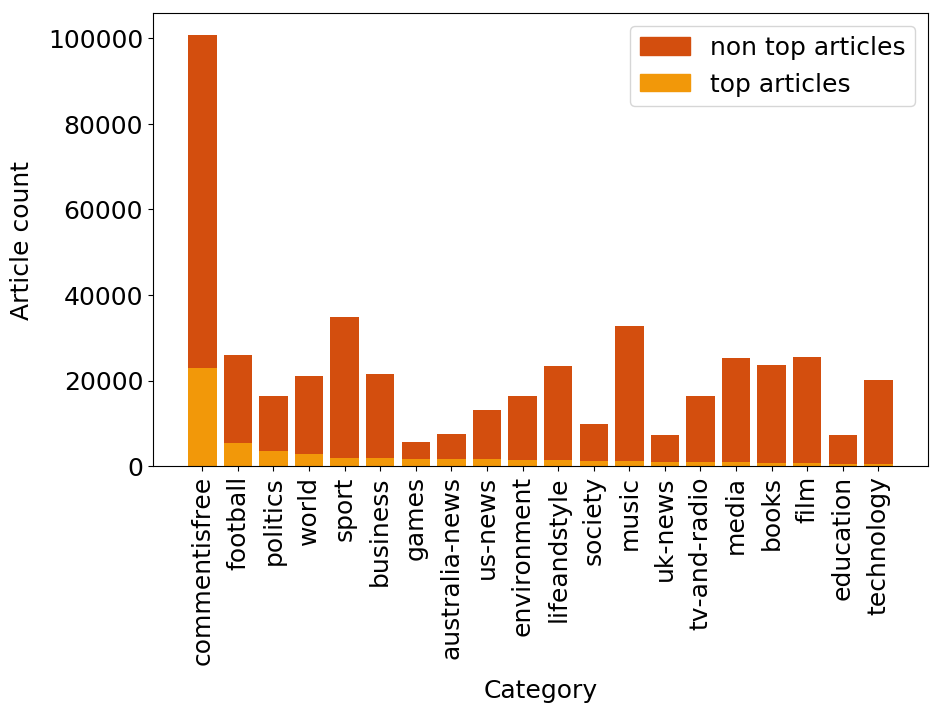
\includegraphics[width=0.45\textwidth]{fig/top_ten_category.png}
	\caption{\textmd{Number of articles for the first $20$ categories containing most of the top articles.}}
	\label{fig:top_ten_category}
\end{figure}

\textit{Model 5} is the worst performing model. Its precision of $0.100$ is just as good as a random prediction.
One reason is that $19\%$ of all articles got released on full hours and might also be due to the fact that \textit{The Guardian} has an international readership spread over multiple time zones. 
Therefore, the time of the day has almost no effect on the number of comments that an article receives as seen in \autoref{fig:top_ten_time}. 
Additionally, the day of the week has also no significant effect on the weekly article performance. 

\begin{figure}[h]
	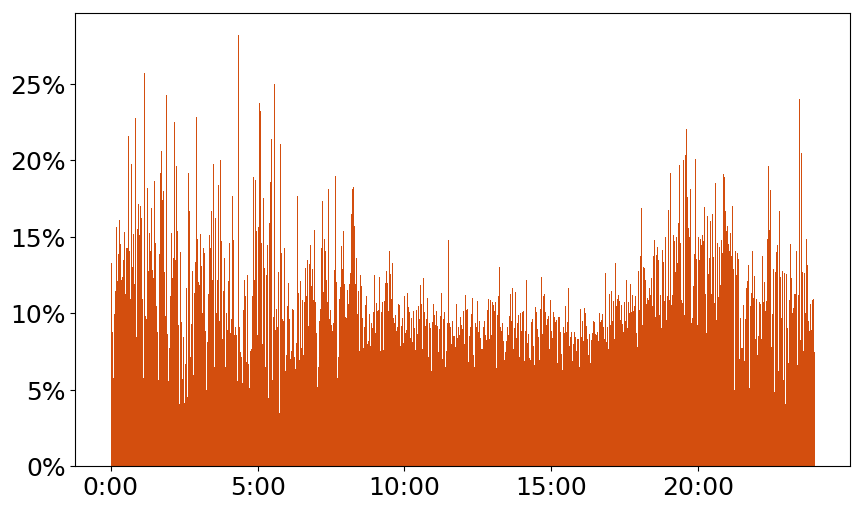
\includegraphics[width=0.45\textwidth]{fig/top_ten_time.png}
	\caption{\textmd{Percentage of top articles per time of the day.}}
	\label{fig:top_ten_time}
\end{figure}

\textit{Model 6} had also a small but slightly better performance than \textit{Model 5}. 
Neither the length of the headline nor the length of the article text is feasible for an accurate prediction.

\textit{Model 7} processes just a single numeric value as input. For a good performance using the competitive score, it would be necessary to be able to divide the values into distinct intervals that can be assigned to each class.
Unfortunately, the competitive score distribution of top articles is similar to the overall distribution of the competitive score.

\subsection{Combined Models}
As seen in \autoref{fig:correlation_matrix}, \textit{Model 1} and \textit{2} correlate the most with a value of $0.589$ which is due to processing the same input feature.
The correlation between \textit{Model 3} and both \textit{Model 1} and \textit{2} is also relatively high because the headline and the first $50$ words of the article probably provide a similar context.

\autoref{tbl:results_combined} shows the results of our combinations. We combine \textit{Model 2} with each other model because it exhibits the best results processing text input and has a low correlation to other models.
\textit{Model 5} which is correlating least with all other models has a very low $F_1$-score. Therefore, we exclude it from our consideration to combine it with every other model.

\begin{table}[]
\centering
\label{tbl:results_combined}
\caption{\textmd{Precision (P), recall (R), and F$_1$-score of all combined models}}
\vspace{-0.2cm}\begin{tabular}{cccc}
\toprule
% \textbf{Features} &
% \specialcellbold{Short description} &
\specialcellbold{Combination} &
\specialcellbold{P} &
\specialcellbold{R} &
\specialcellbold{F$_1$} \\
\midrule
2 3 & .224 & .645 & .323\\
2 4 & .245 & .627 & .342\\
2 5 & .227 & .581 & .317 \\
2 6 & .217 & .651 & .317\\
2 7 & .214 & .625 & .311\\
3 4 & .252 & .577 & .339\\
2 3 4 & .265 & .607 & .357\\
\bottomrule
\end{tabular}
\end{table}

The combination of \textit{Model 2} with each \textit{Model 5}, \textit{6}, and \textit{7} doesn't have a better performance than \textit{Model 2} itself. 
Thus, we notice that the publishing time, text metrics, and competitive score are unqualified additional features for the headline text.

Combining each \textit{Model 3} and \textit{4} with \textit{Model 2} shows performance improvements.
Consequently, we combine these models and receive our best \textit{precision} and $F_1$-score.

Compared to other approaches (\autoref{tbl:compare_approaches}), our $F_1$-score is $42\%$ higher than the  value by Tsagikas et al. and $5\%$ smaller than the values presented by Ambroselli et al. \cite{ambroselli2018prediction}.

\begin{table}[h]
\centering
\caption{\textmd{Precision (P), recall (R), and F$_1$-score of baseline approaches and our approach.}}
\label{tbl:compare_approaches}
\vspace{-0.2cm}\begin{tabular}{lccc}
\toprule
\specialcellbold{Approach} &
\specialcellbold{P} &
\specialcellbold{R} &
\specialcellbold{F$_1$} \\
\midrule
Tsagkias et al. & .16 & .72 & .26\\
Ambroselli et al. & .26 & .75 & .39\\
Our Approach & .27 & .61 & .37\\
\bottomrule
\end{tabular}
\end{table}

Finally, we point out that our results were achieved by using another dataset than Ambroselli et al. 
Their data contains only articles by a German magazine. 
Due to the English readership, \textit{The Guardian} releases its articles internationally which implies a much broader audience and discussed topics need to address this diversity. Consequently, to compare both approaches in a more appropriate way, it would be necessary to execute them on the same dataset.

Further classification improvements could be achieved by using a more sophisticated network architecture. A recent research approach by Conneau et al. shows that a very deep CNN architecture using character embeddings can be used for text classification \cite{conneau2016very}. Applying this method might lead to a better semantically interpretation of the text features and could result in more precise prediction.